%V ďalšej časti prezentujte vlastný prínos a vlastné výsledky porovnajte s výsledkami iných. Charakterizujte použité metódy.
%Vyhýbajte sa používaniu žargónu.
%Používajte starú múdrosť: 1 obrázok je viac než 1000 slov.

\subsection{Comparison of Models} 
\label{sec:results-comparison}

TODO: Introduce shortcuts and add references to descriptions. \\

\subsubsection{4-2-4 Encoder}
\ref{sec:datasets-auto4} 

For all our models \ref{sec:our-models} tested on the 4-2-4 encoder task~\ref{sec:datasets-auto4} TLR~\ref{sec:our-tlr} had the best success rate. 

For TLR, BAL, GeneRec, BP, CHL, other learning rules

\begin{table}
  \centering
    \begin{tabular}{|l|l|l|l|l|}
    \hline
    Algorithm&$\lambda$&Success&Epcs&SEM \\
    \hline
    BP&2.4&100&60&5.1\\
    \hline
    AP&2.8&100&54&3.6\\
    \hline
    GR&0.6&90&418&28\\
    \hline
    GR Sym&1.4&56&88&2.9\\
    \hline
    GR Mid&2.4&92&60&3.4\\
    \hline
    CHL&1.2&56&77&1.8\\
    \hline
    BAL&0.9&65&1000&\\
    \hline
    BAL TLR&0.0002 | 500&94&8251&\\
    \hline
    BAL Recirc&0.7&34&10000&\\
    \hline
    \end{tabular}
  \caption{Comparing performance of different models on the \emph{4-2-4 encoder} task.} 
  \label{tab:results-cmp-auto4}
\end{table}

\paragraph{Hidden activations.}
\ref{sec:our-hidden-activation}  

%===== TODO hidden activation timelines with commentaries (for TLR, BAL, GeneRec) 
% 2x success, 2x error (wrong settle, divergence) 

\begin{figure}[H]
  \centering
  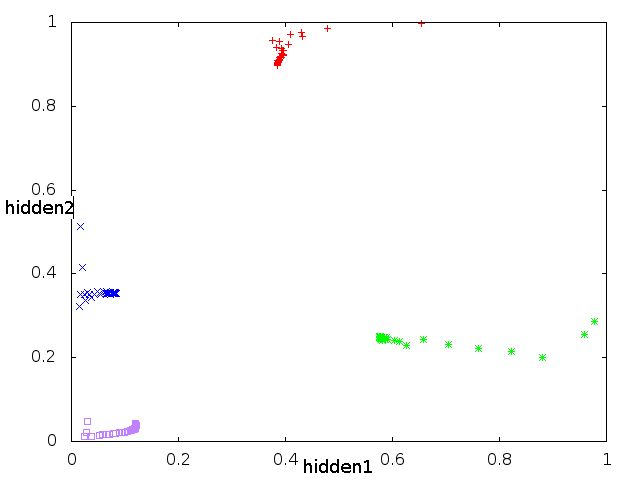
\includegraphics[width=0.45\textwidth]{../presentation/img/nice.png}   
  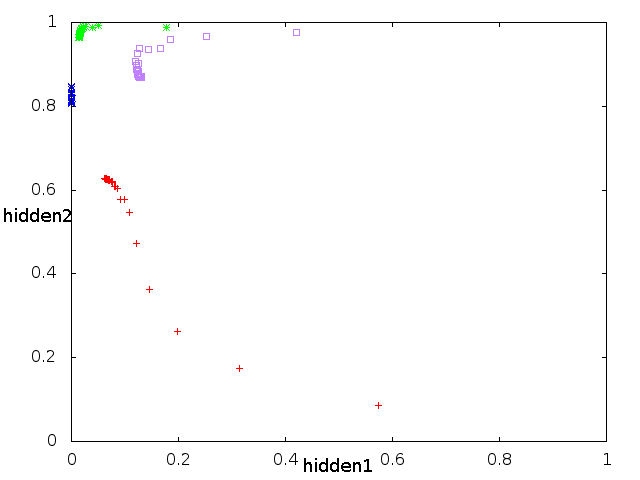
\includegraphics[width=0.45\textwidth]{../presentation/img/left_top.png}    
  \caption{BAL hidden activations on the \emph{4-2-4 encoder} for successfull networks.}
  \label{fig:results-hidden-activations-bal-good}
\end{figure}

\begin{figure}[H]
  \centering
  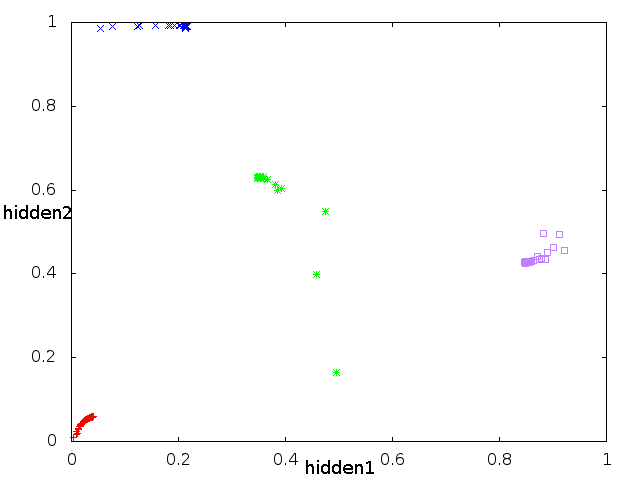
\includegraphics[width=0.45\textwidth]{../presentation/img/tazisko.png}   
  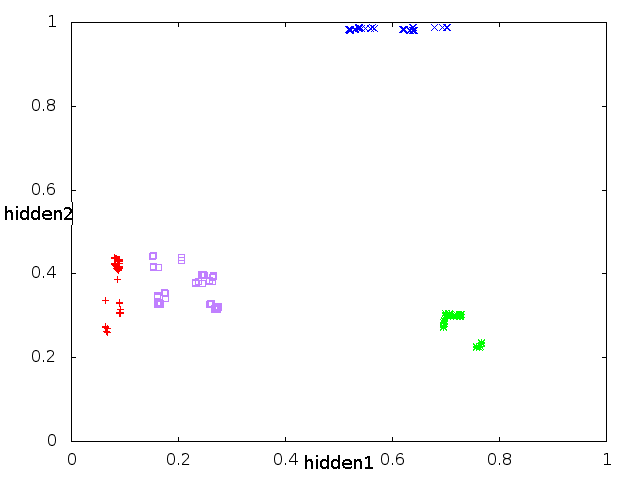
\includegraphics[width=0.45\textwidth]{../presentation/img/non-convergent.png}    
  \caption{BAL hidden activations on the \emph{4-2-4 encoder} for {\bf not} successfull networks. On the left image the network settled with constant hidden activations for which the resulting tw--dimensional task is not linearly separable. On the right image the network failed to convergence swtich several hidden activation states.}
  \label{fig:results-hidden-activations-bal-bad}
\end{figure}


\subsubsection{Complex Binary Vector Associations}
\ref{sec:datasets-k3} 

%===== TODO table: best parameter setting networks with hidden.size= constant (success, epoch, stddev) / model \\

\paragraph{Different hidden sizes.} 

\subsubsection{Hand--written digits}
\ref{sec:datasets-digits} 

TODO simulation + plots \ref{sec:datasets-digits} 

For TLR, BAL, GeneRec + known performers 
TODO: table: best parameter setting networks with hidden.size= constant (success, epoch, stddev) / model \\

\paragraph{Backward representations.} 
\ref{sec:our-backward-repre} 

TODO 3x 10x backward digit representations 

\begin{figure}[H]
  \centering
  
\includegraphics{../presentation/img/dig_0.png} 
  
\includegraphics{../presentation/img/dig_1.png} 
  
\includegraphics{../presentation/img/dig_2.png} 
  
\includegraphics{../presentation/img/dig_3.png} 
  
\includegraphics{../presentation/img/dig_4.png} 
  
\includegraphics{../presentation/img/dig_5.png} 
  
\includegraphics{../presentation/img/dig_6.png} 
  
\includegraphics{../presentation/img/dig_7.png} 
  
\includegraphics{../presentation/img/dig_8.png} 
  
\includegraphics{../presentation/img/dig_9.png} 
  \caption{Backward representations on \emph{digits} for GeneRec.}
  \label{fig:results-backward-repre-generec}
\end{figure}
